\documentclass[10pt,a4paper]{article}

\usepackage[T1]{fontenc}
\usepackage[utf8]{inputenc}
\usepackage{lmodern}
\usepackage[margin=1.62cm]{geometry}
\usepackage{setspace}
\usepackage{amsmath,amssymb,mathtools}
\usepackage{booktabs}
\usepackage{tikz}
\usetikzlibrary{arrows.meta,positioning}
\usepackage{enumitem}
\usepackage{caption}
\usepackage{hyperref}
\hypersetup{colorlinks=true,linkcolor=black,citecolor=black,urlcolor=blue}

\setstretch{1.07}
\setlength{\parskip}{0.34em}
\setlength{\parindent}{1.05em}
\setlist{nosep,leftmargin=1.2em}

\newcommand{\cmax}{C_{\max}}
\newcommand{\Prob}{\mathbb{P}}

\title{\large Research for Solving Breakdown Risk in School Bag Factory Scheduling by Using Status-Synchronized Digital Twin Coordination}
\author{Computer Science Short Paper\\Companion to the system-design thesis}
\date{October 2026}

\begin{document}
\maketitle
\vspace{-1.6em}

\begin{abstract}
\noindent
Machine status in a school-bag factory is not a label beside the schedule. Cutter wear and needle heat change the next cycle time, the energy, and the chance that the cycle is interrupted. This paper presents status-synchronized digital twin coordination with chance constraints (SSDT-CC). A live health state scales processing time, a hazard gives a failure probability, and an assignment whose probability exceeds a tolerance is not deleted: a sixteen-minute preventive maintenance renews the machine and the cycle is recomputed. The dispatcher is called again whenever a resource becomes free, so the twin reschedules by rewriting the state the score reads. On twenty accelerated-wear order books the coupled system finishes in \(1122\) minutes with \(0.81\) expected failures, against about \(2059\) minutes and \(39\) expected failures for earliest due date. A tolerance sweep shows that a tighter limit buys fewer failures with more maintenance. The plant uses expected delay, not a noisy sensor.
\end{abstract}

\section{Introduction}

Condition-based maintenance and digital twins are usually described as monitoring systems. A remaining-useful-life model estimates when a tool will cross a failure threshold \cite{si2011,lei2018}. A twin mirrors the machine for an operator or for a planner who still writes the sequence by hand \cite{grieves2017,tao2019,lee2015}. Scheduling research has started to put degradation inside flexible job shops \cite{cbm2024}, most often as a cost or as a constraint on a plan that is built once. End-to-end multitarget policies \cite{wang2025} still act on operation--machine pairs and do not renew a worn tool.

A school-bag shift does not offer that separation. The automatic cutter begins the day already worn. Running it makes it slower, hotter, and more likely to stop. A schedule that treats processing time as a constant from the routing sheet is using a health factor of one, whatever number is displayed on a screen. Inserting maintenance on a clock, independently of which orders are waiting, spends the tool change on a machine the book does not need and withholds it from a machine the book is about to overload.

The contribution is a closed loop with one action. Health is the twin. The chance constraint is the veto. The action, when the veto fires, is a short renewal of that same machine, after which the dispatcher scores the shop again. The score that chooses among bundles is the resource-coupled graph policy of the companion thesis. This paper isolates what the health loop adds: the maps from health to time, energy, and failure, the maintenance rewrite, and the estimates obtained when that rewrite is allowed or forbidden.

\section{Health, time, energy, and hazard}

Each machine \(k\) carries a scalar health \(h_k\). Zero is a new tool. One is a tool the maintenance standard calls failed. Between decisions the design model is a Wiener drift,
\begin{equation}
\mathrm{d}h_k = \eta_k\,\mathrm{d}t + \sigma_k\,\mathrm{d}B_t ,
\label{eq:sde}
\end{equation}
observed through a noisy indicator \(y_k = h_k + \epsilon_k\). A Kalman filter would predict \(\hat h^- = \hat h + \eta_k p\), then correct with the reading \cite{kalman1960}. The estimation plant has no sensor noise. It applies the drift directly,
\begin{equation}
h_k \leftarrow \min(1.25,\; h_k + \eta_k p),
\label{eq:wear}
\end{equation}
which is the Kalman prediction with posterior variance held at zero. For the automatic cutter, \(\eta = 0.00115\) per minute and the day starts at \(h = 0.58\).

Processing time uses the health factor \(1 + 0.85\, h^{1.15}\). The exponent above one makes the last part of the wear more expensive than the first. Energy of a cycle is
\begin{equation}
E = P_k \cdot \frac{p}{60} \cdot (1 + 0.45\, h_k),
\label{eq:energy}
\end{equation}
in kilowatt-hours, with \(P_k\) the rated power. Expected repair energy is charged separately at half power for an expected repair of \(48\) minutes.

The failure probability is an intensity, not a Gaussian crossing. Mid-cycle health is \(h_{\mathrm{mid}} = h + \tfrac12 \cdot 0.0004 \cdot p\), and
\begin{equation}
\lambda = 2.4 \big(\max(0, h_{\mathrm{mid}} - 0.40)\big)^{1.35},
\qquad
\phi = 1 - \exp(-\lambda \, p/60).
\label{eq:phi}
\end{equation}
Below health \(0.40\) the intensity is zero. Above it, intensity grows faster than linearly. The expected breakdown delay charged to the machine is \(48\phi\) minutes. The plant does not draw a Bernoulli failure. Methods are compared on the risk they choose to accept, which is reproducible.

A Gaussian ceiling gives a different veto. The probability of crossing a limit during the cycle can sit under the tolerance while \eqref{eq:phi} sits over it. On the worn cutter the two tests disagree: the hazard vetoes at \(\varepsilon = 0.10\) and a Gaussian ceiling at \(0.90\) would still allow the cycle. The dispatcher uses the hazard, and the thesis records the disagreement rather than averaging the two tests.

\section{Chance-constrained renewal}

An assignment is refused in its current form when \(\phi > \varepsilon\) or when the predicted health at the end of the cycle exceeds \(0.90\). The default tolerance is \(\varepsilon = 0.10\). Refusal does not remove the machine from the feasible set. The same bundle is offered with a preventive maintenance prefixed,
\begin{equation}
h_k \leftarrow 0.30\, h_k + 0.04,
\qquad
\Delta \leftarrow \Delta + 16.
\label{eq:pm}
\end{equation}
Time, energy, and \(\phi\) are recomputed at the renewed health. The sixteen minutes occupy the machine and the operator. They do not hold the die or the thread lot. The factor \(0.30\) is a partial renewal: a knife or needle change brings the indicator down and leaves a residual of \(0.04\). On a machine that is already healthy the map barely moves \(h\), \(\phi\) is already zero, and the test does not fire.

\begin{figure}[ht]
\centering
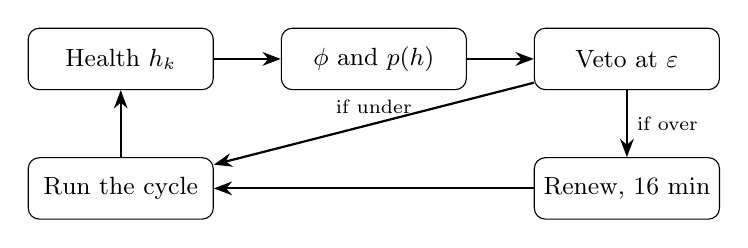
\begin{tikzpicture}[
  box/.style={draw, rounded corners, align=center, font=\small, minimum width=2.35cm, minimum height=0.78cm},
  arr/.style={-{Stealth}, thick}
]
\node[box] (h) {Health \(h_k\)};
\node[box, right=0.85cm of h] (phi) {\(\phi\) and \(p(h)\)};
\node[box, right=0.85cm of phi] (dec) {Veto at \(\varepsilon\)};
\node[box, below=0.85cm of dec] (pm) {Renew, \(16\) min};
\node[box, below=0.85cm of h] (run) {Run the cycle};
\draw[arr] (h) -- (phi);
\draw[arr] (phi) -- (dec);
\draw[arr] (dec) -- node[right, font=\scriptsize] {if over} (pm);
\draw[arr] (dec) -- node[above, font=\scriptsize] {if under} (run);
\draw[arr] (pm) -- (run);
\draw[arr] (run) -- (h);
\end{tikzpicture}
\caption{The twin writes health, the hazard tests the next cycle, and either maintenance or ordinary wear writes health again. The dispatcher is called when the resource is next free.}
\label{fig:loop}
\end{figure}

Figure~\ref{fig:loop} is the whole coordination loop. There is no second solver that rebuilds a Gantt chart from scratch. Because candidates are rebuilt whenever a machine and an operator are free, a health value written at the last completion is already inside the next score. A rush order enters the same rebuild when its release time arrives. Rescheduling is the dispatch itself.

On one navy shell the arithmetic is local and unfavourable to maintenance. Cutter-A at \(h = 0.58\) takes \(27.3\) minutes, uses about \(3.90\,\mathrm{kWh}\), and has \(\phi = 0.106\), so the expected repair delay is \(5.1\) minutes. The total occupation if the risk is accepted is about \(32.4\) minutes. Maintenance renews health to \(0.214\), cuts the processing time to \(21.5\) minutes, and adds \(16\) minutes, for an occupation of \(37.5\) minutes and \(4.65\,\mathrm{kWh}\), with \(\phi = 0\). The manual cutter, already healthy, takes \(37.3\) minutes and \(1.64\,\mathrm{kWh}\) with no failure. One cycle does not pay for the tool change. Three unrepaired cuts on the same automatic cutter charge about \(102\) minutes and end near health \(0.68\). One renewal followed by three cuts charges about \(82\) minutes. The saving appears across cycles, which is why the estimate below is a day and not a row.

\section{Estimate on the worn day}

The cell has nine machines and eight operators. Cutter-A, Lockstitch-2, and the embroidery head start the nominal day at health \(0.58\), \(0.52\), and \(0.46\). The accelerated-wear scenario adds \(0.10\) to every initial health and multiplies every wear coefficient by \(1.85\). All methods share the mask. RCH is the graph score with the maintenance test off. RCH-SSDT is the same score with the test on. ``No status'' zeroes health and failure inside the score and does not maintain. Means are over twenty paired books.

\begin{table}[ht]
\centering
\caption{Accelerated wear, twenty books. Times are minutes. Energy is kilowatt-hours. PM is the mean number of renewals.}
\label{tab:wear}
\small
\begin{tabular}{lrrrrrr}
\toprule
Method & Makespan & Tardiness & On time & Energy & Failures & PM \\
\midrule
FIFO & 2097.7 & 5898.7 & 0.397 & 388.2 & 42.26 & 0 \\
EDD & 2059.3 & 1849.0 & 0.584 & 384.3 & 38.75 & 0 \\
RCH & 1782.0 & 895.1 & 0.697 & 310.0 & 30.58 & 0 \\
No status & 1676.9 & 1054.7 & 0.706 & 283.6 & 28.88 & 0 \\
RCH-SSDT & 1121.7 & 287.2 & 0.850 & 176.1 & 0.81 & 11.95 \\
\bottomrule
\end{tabular}
\end{table}

Seeing wear without being allowed to renew it is worth several hundred minutes: RCH and the no-status ablation finish near \(1700\)--\(1780\) minutes with about thirty expected failures, against about \(2100\) minutes and about forty failures for the rules. Renewal is the second cut. Twelve maintenances cost \(192\) minutes of tool-change time. Expected repair delay avoided, relative to earliest due date, is on the order of \(1800\) minutes. Makespan falls to \(1122\), energy to \(176\,\mathrm{kWh}\), and expected failures to \(0.81\). Tardiness falls from \(1849\) to \(287\) minutes. On this scenario the due-date gap is large beside the spreads (\(364\) minutes for the full system, about \(1000\) for earliest due date), because the failures a due-date rule accepts are what make the orders late.

The same pattern appears on an ordinary day, with a smaller maintenance count. Over twenty nominal books the coupled system finishes in \(1052\) minutes and \(168\,\mathrm{kWh}\) with \(0.91\) expected failures and \(5.4\) renewals. The graph score alone, which can prefer the healthy cutter and cannot renew the worn one, finishes in \(1234\) minutes and \(211\,\mathrm{kWh}\) with \(10.1\) expected failures. Status features without the maintenance action reproduce that first band, not the second.

Table~\ref{tab:eps} repeats the wear stress on eight further books while \(\varepsilon\) changes. These seeds are not the twenty books of Table~\ref{tab:wear}. Tightening the tolerance from \(0.50\) to \(0.02\) raises the maintenance count from \(7.0\) to \(15.0\), drops expected failures from \(9.77\) to \(0.05\), and on this parameterization also shortens the day and lowers energy. The curve has not yet turned upward. A longer tool change, or a fleet that is already healthy, would make excessive maintenance expensive. The useful fact is that \(\varepsilon\) is a visible knob. A scheduler that hides the tolerance inside a trained weight cannot be retuned when the knife-change time changes.

\begin{table}[ht]
\centering
\caption{Tolerance sweep on eight accelerated-wear books. The policy is the coupled system.}
\label{tab:eps}
\small
\begin{tabular}{lrrrr}
\toprule
\(\varepsilon\) & Makespan & Failures & Energy & PM \\
\midrule
0.02 & 1145.3 & 0.046 & 182.0 & 15.00 \\
0.05 & 1151.3 & 0.238 & 182.3 & 13.88 \\
0.10 & 1170.2 & 0.813 & 195.7 & 12.63 \\
0.20 & 1187.2 & 2.741 & 198.2 & 10.38 \\
0.50 & 1335.7 & 9.773 & 228.6 & 7.00 \\
\bottomrule
\end{tabular}
\end{table}

\section{Why the local loss and the daily gain coexist}

Table~\ref{tab:one} puts the three ways of cutting one navy shell on one line. Maintenance is the slowest immediate occupation and uses more energy than the manual cutter. It is the only option that both uses the fast machine and leaves that machine below the hazard threshold.

\begin{table}[ht]
\centering
\caption{One navy shell. Times are minutes. Energy is kilowatt-hours. Extra is expected repair delay, or the sixteen-minute renewal.}
\label{tab:one}
\small
\begin{tabular}{lrrr}
\toprule
Option & Process & Extra & Energy \\
\midrule
Cutter-A, accept \(\phi = 0.106\) & 27.3 & 5.1 & 3.90 \\
Cutter-A, renew first & 21.5 & 16.0 & 4.65 \\
Cutter-B, already healthy & 37.3 & 0.0 & 1.64 \\
\bottomrule
\end{tabular}
\end{table}

The day is a sequence of such rows that share a health state. Three unrepaired cuts on Cutter-A charge about \(102\) minutes and finish near health \(0.68\), where the next shell is both slower and more likely to fail. One renewal and then three cuts charge about \(82\) minutes and stay near the renewed health. Twelve such renewals on a worn book are \(192\) minutes of tool-change time. The repair delay they avoid, relative to a due-date rule that never renews, is on the order of \(1800\) minutes. The local row and the daily table are not in conflict. They answer different questions: whether this cycle, alone, is shorter with a knife change, and whether the shift is shorter if worn cycles are allowed to compound.

The same split is visible without accelerating wear. On twenty ordinary books the coupled system uses \(5.4\) renewals and finishes in \(1052\) minutes with \(0.91\) expected failures. The graph score, allowed to see health and forbidden to renew, finishes in \(1234\) minutes with \(10.1\) expected failures. Zeroing health inside the score and forbidding renewal lands in that same band, not in the renewed one. A penalty on a worn machine can steer work toward the healthy cutter. It cannot put the automatic cutter back into the pool at health \(0.21\). Only the rewrite in \eqref{eq:pm} does that, which is why the tolerance in Table~\ref{tab:eps} is a maintenance count and not merely a reweighting of \(\psi\).

\section{What this estimate includes}

The tables use the hazard \eqref{eq:phi}, the renewal \eqref{eq:pm}, and the deterministic wear recursion \eqref{eq:wear}. They do not use a random breakdown draw, so a second run with the same seeds reproduces the means. They do not use the Kalman correction. A noisy current or temperature would be reduced to the unit interval and then filtered; until that residual exists, filtering it would be theatre. They also do not train a deep network. The dispatcher that proposes the bundle is the identified one-hop score of the companion paper, and the twin's only extra authority is the maintenance bit on that bundle.

An ordinary book, included so the wear table is not the only evidence, finishes under the coupled system in \(1052\) minutes and \(168\,\mathrm{kWh}\) with \(0.91\) expected failures and \(5.4\) renewals. First-in-first-out on the same twenty books takes \(1521\) minutes and \(303\,\mathrm{kWh}\) with \(18.0\) expected failures and no renewals. The graph score without renewal sits between them, at \(1234\) minutes, \(211\,\mathrm{kWh}\), and \(10.1\) expected failures. Health-aware dispatch and health renewal are different levers. The second lever is the one this paper isolates, and it is the one that moves failures from the teens, or from about thirty on a worn day, to under one.

\section{Conclusion}

SSDT-CC keeps machine health inside the dispatch loop of a school-bag shop. The health state scales time and energy, a hazard supplies the failure probability, and a chance constraint inserts a sixteen-minute partial renewal instead of deleting the worn machine. One cycle does not repay the renewal. A worn day does: about twelve renewals replace on the order of thirty expected failures and several hundred minutes of makespan. The Kalman update is the form to use when a sensor is noisy. The tables were produced with a deterministic wear recursion, so they estimate the chosen risk and not a particular factory's next breakdown.

\begin{thebibliography}{99}
\bibitem{lee2015} J.~Lee, B.~Bagheri, and H.-A. Kao. A cyber-physical systems architecture for Industry 4.0-based manufacturing systems. \emph{Manufacturing Letters}, 3:18--23, 2015.
\bibitem{grieves2017} M.~Grieves and J.~Vickers. Digital twin: Mitigating unpredictable, undesirable emergent behavior in complex systems. In \emph{Transdisciplinary Perspectives on Complex Systems}, pp.~85--113. Springer, 2017.
\bibitem{tao2019} F.~Tao, H.~Zhang, A.~Liu, and A.~Y.~C. Nee. Digital twin in industry: State-of-the-art. \emph{IEEE Transactions on Industrial Informatics}, 15(4):2405--2415, 2019.
\bibitem{qi2018} Q.~Qi and F.~Tao. Digital twin and big data towards smart manufacturing and Industry 4.0: 360 degree comparison. \emph{IEEE Access}, 6:3585--3593, 2018.
\bibitem{si2011} X.-S. Si, W.~Wang, C.-H. Hu, and D.-H. Zhou. Remaining useful life estimation -- a review on the statistical data driven approaches. \emph{European Journal of Operational Research}, 213(1):1--14, 2011.
\bibitem{lei2018} Y.~Lei, N.~Li, L.~Guo, N.~Li, T.~Yan, and J.~Lin. Machinery health prognostics: A systematic review from data acquisition to RUL prediction. \emph{Mechanical Systems and Signal Processing}, 104:799--834, 2018.
\bibitem{gebraeel2005} N.~Z. Gebraeel, M.~A. Lawley, R.~Li, and J.~K. Ryan. Residual-life distributions from component degradation signals: A Bayesian approach. \emph{IIE Transactions}, 37(6):543--557, 2005.
\bibitem{kalman1960} R.~E. Kalman. A new approach to linear filtering and prediction problems. \emph{Journal of Basic Engineering}, 82(1):35--45, 1960.
\bibitem{charnes1959} A.~Charnes and W.~W. Cooper. Chance-constrained programming. \emph{Management Science}, 6(1):73--79, 1959.
\bibitem{birge2011} J.~R. Birge and F.~Louveaux. \emph{Introduction to Stochastic Programming}. Springer, 2nd edition, 2011.
\bibitem{cbm2024} L.~Li, L.~Deng, B.~Tang, and F.~Wang. Bi-objective flexible job shop scheduling on machines considering condition-based maintenance activities. \emph{Proceedings of the Institution of Mechanical Engineers, Part O: Journal of Risk and Reliability}, 238(6):1244--1255, 2024.
\bibitem{wang2025} R.~Wang, Y.~Jing, C.~Gu, S.~He, and J.~Chen. End-to-end multitarget flexible job shop scheduling with deep reinforcement learning. \emph{IEEE Internet of Things Journal}, 12(4):4420--4434, 2025.
\bibitem{monostori2016} L.~Monostori et al. Cyber-physical systems in manufacturing. \emph{CIRP Annals}, 65(2):621--641, 2016.
\bibitem{koren2010} Y.~Koren and M.~Shpitalni. Design of reconfigurable manufacturing systems. \emph{Journal of Manufacturing Systems}, 29(4):130--141, 2010.
\end{thebibliography}

\end{document}
